\begin{Shaded}
\begin{Highlighting}[]
\OperatorTok{\%\%}\NormalTok{html}
\end{Highlighting}
\end{Shaded}

\hypertarget{methods}{%
\section{Methods}\label{methods}}

The practical implemntation of what is described in this section is
available as a Python package called Koala (Kitaev On Amorphous
LAttices) \textcite{tomImperialCMTHKoalaFirst2022} most of the figures
shown were generated with Koala.

\hypertarget{voronisation}{%
\subsection{Voronisation}\label{voronisation}}

In order to study the properties of the amorphous Kitaev model we need a
way to sample from the space of possible trivalent graphs.

A very simple way to do this is to use a Voronoi partition of the torus.
We start by sampling \emph{seed points} uniformly (or otherwise) on the
torus. We then compute the partition of the torus into regions closest
(with a Euclidean metric) to each seed point. The straight lines (if the
torus is flattened out) at the borders of these regions become the edges
of the new lattice and the points where they intersect beceme the
vertices.

The graph generated by a Voronoi partition of a two dimensional surface
is always planar meaning that no edges cross eachother when the graph is
embedded into the plane. It is also trivalent in the sense that every
vertex is connected to exactly three edges \textbf{cite}.

Ideally we might instead sample uniformly from the space of possible
trivalent graphs, and indeed there has been some work on how to do this
using a Markov Chain Monte Carlo approach
\textcite{alyamiUniformSamplingDirected2016}, however it does not
gurantee that the resulting graph is planar which we will need to ensure
that the edges can be 3-coloured.

In practice, we then use a standard algorithm
\textcite{barberQuickhullAlgorithmConvex1996} from scipy
\textcite{virtanenSciPyFundamentalAlgorithms2020a} which actually
computes the Voronoi partition of the plane. In order to compute the
Voronoi partition of the torus, I take the seed points and replicate
them into a repeating grid, either 3x3 (or for very small numbers of
seed points 5x5). I then identify edges in the output to construct a
lattice on the torus.

\begin{figure}
\hypertarget{fig:lattice_construction_animated}{%
\centering
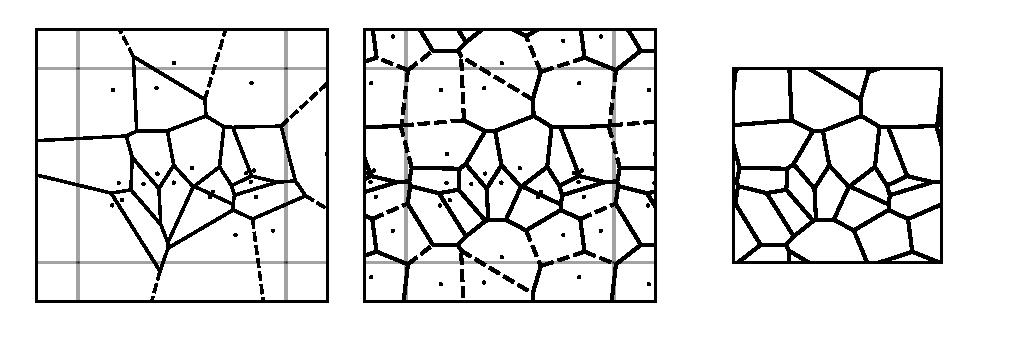
\includegraphics{figure_code/amk_chapter/lattice_construction_animated/lattice_construction_animated.pdf}
\caption{(Left) Lattice construction begins with the Voronoi partition
of the plane with respect to a set of seed points (black points) sampled
uniformly from \(\mathbb{R}^2\). (Center) However we actually want the
Voronoi partition of the torus so we tile the seed points into a three
by three grid. The boundaries of each tile are shown in light grey.
(Right) Finally we indentify edges correspond to each other across the
boundaries to produce a graph on the torus. An edge colouring is shown
here to help the reader identify corresponding
edges.}\label{fig:lattice_construction_animated}
}
\end{figure}

\hypertarget{graph-representation}{%
\subsection{Graph Representation}\label{graph-representation}}

We represent the graph structure with an ordered list of edges \((i,j)\)
so we can represent both directed and undirected graphs which is useful
for defining the sign of bond operators \(u_{ij} = - u_{ji}\).

\hypertarget{coloring-the-bonds}{%
\subsection{Coloring the Bonds}\label{coloring-the-bonds}}

The Kitaev model requires that each edge in the lattice be assigned a
label \(x\), \(y\) or \(z\) such that each vertex has exactly one edge
of each type connected to it. Let \(\Delta\) be the maximum degree of a
graph which in our case is 3. If \(\Delta > 3\) it is obviously not
possible to 3 color the edges but the general theory of when this is and
isn't possible for graphs with \(\Delta \leq 3\) is more subtle.

In the graph theory literature, graphs where all vertices have degree 3
are commonly called cubic graphs, there is no term for graphs with
maximum degree 3. Planar graphs are those that can be embedded onto the
plane without any edges crossing. Bridgeless graphs do not contain any
edges that, when removed, would partition the graph into disconnected
components.

It's important to be clear that this problem is different from that
considered by the famous 4 color theorem
\textcite{appelEveryPlanarMap1989} . The 4 color thorem is concerned
with assiging colours to the \textbf{vertices} of a graph such that no
vertices that share an edge are the same colour. Here we are concerned
with an edge colouring.

The four color theorem applies to planar graphs, those that can be
embedded onto the plane without any edges crossing. Here we are actually
concerned with Toroidal graphs which can be embedded onto the torus
without any edges crossing. In fact toroidal graphs require up to 7
colors \textcite{heawoodMapColouringTheorems} . The complete graph
\(K_7\) is a good example of a toroidal graph that requires 7 colours.

\(\Delta + 1\) colours are enough to edge-colour any graph and there is
an \(\mathcal{O}(mn)\) algorithm to do it for a graph with \(m\) edges
and \(n\) vertices \textcite{gEstimateChromaticClass1964}. Restricting
ourselves to graphs with \(\Delta = 3\) like ours, those can be
4-edge-coloured in linear time
\textcite{skulrattanakulchai4edgecoloringGraphsMaximum2002} .

It's trickier if we want to 3-edge-colour them however. Cubic, planar
bridgeless graphs can be 3-edge-coloured if and only if they can be
4-face-coloured \textcite{tait1880remarks} . For which there is an
\(\mathcal{O}(n^2)\) algorithm robertson1996efficiently . However it is
not clear whether this extends to cubic, \textbf{toroidal} bridgeless
graphs.

\hypertarget{face-colourablity-implies-3-edge-colourability}{%
\paragraph{4-face-colourablity implies
3-edge-colourability}\label{face-colourablity-implies-3-edge-colourability}}

The proof of that 4-face-colourablity implies 3-edge-colourability can
be sketched out quite easily: 1. Assume the faces of G can be 4-coloured
with labels (0,1,2,3) 2. Label each edge of G according to
\(i + j \mathrm{mod} 3\) where i and j are the labels of the face
adjacent to that edge. For each edge label there are two face label
pairs that do not share any face labels. i,e the edge label \(0\) can
come about either from faces \(0 + 3\) or \(1 + 2\).

\[\begin{align}
0 + 3 \;\mathrm{or}\; 1 + 2 &= 0 \;\mathrm{mod}\; 3\\ 
0 + 1 \;\mathrm{or}\; 2 + 3 &= 1 \;\mathrm{mod}\; 3\\
0 + 2 \;\mathrm{or}\;1 + 3 &= 2 \;\mathrm{mod}\; 3\\
\end{align}
\]

\begin{enumerate}
\def\labelenumi{\arabic{enumi}.}
\setcounter{enumi}{2}
\tightlist
\item
  In a cubic planar G, a vertex v in G is always part of 3 faces and the
  colors of those faces determines the colors of the edges that connect
  to v. The three faces must take three distinct colors from (0,1,2,3).
\item
  From there's easy to convince yourself that those three distinct face
  colours can never produce repeated edge colours according to the
  \(i+j \;\mathrm{mod}\; 3\) rule.
\end{enumerate}

This implies that all cubic planar graphs are 3-edge-colourable. It does
not apply to toroidcal graphs, however I have not yet generated a
voronoi lattices on the torus that is not 3-edge-colourable. This
suggests that perhaps voronoi lattices have additional structure that
makes them 3-edge-colourable. Intuitively, the kinds of toroidal graphs
that cannot be 3-edge-coloured look as if they could never be generated
by a voronoi partition with more than a few seed points.

\hypertarget{finding-lattice-colourings-in-practice-unfinished}{%
\subsubsection{Finding Lattice colourings in practice
(unfinished)}\label{finding-lattice-colourings-in-practice-unfinished}}

Some things are harder in theory than in practice. 3-edge-colouring
cubic toroidal graphs appears to be one of those things.

The approach I take is relatively standard in the computer science
community for solving NP problems computationally. I don't believe this
problem to be in NP but I tried it anyway.

The trick is to map the problem on into a Boolean Satisfiability `SAT'
problem, use an off the shelf solver for such problems then map the
problem back to the original domain. While SAT solvers are very general,
they are also highly optimised and they do seem to yield good results
for this problem.

SAT solvers encode problems as constraints on some number of boolean
variables \(x_i \in {0,1}\). The constraints must Conjunctive Normal
Form (CNF). CNF means the constraints are encoded as a set of clauses of
the form \[x_1 \;\textrm{or}\; \bar{x}_3 \;\textrm{or}\; x_5\] that
containt logical ORs of some subset of the variables where any of the
variables may also be logical NOT'd which I represent by over bars here.

A solution of the problem is one that makes all the clauses
simultaneously true.

I encode the edge colouring problem as a set of statements about a set
of boolean variables \(x_i \in {0,1}\). For \(B\) bonds we take the
\(3B\) variables \(x_{i\alpha}\) where \(x_{i\alpha} = 1\) indicates
that edge \(i\) has colour \(\alpha\).

For edge colouring graphs we need two kinds of constraints: 1. Each edge
is exactly one colour. 2. No neighbouring edges are the same color.

The first constraint is a kind of artifact of doing this mapping over to
boolean variables, the solver doesn't know anything about the structure
of the problem unless it is encoded into the variables.

The second constraint encodes the structure of the graph itself and can
be constructed easily from the adjacency matrix.

I'll fill in the encoding later but the gist is that we can give this to
a solver and get back: whether the problem is solveable, a solution or
all the possible solutions. Finding a solution is relatively fast, while
finding all the solutions is slower since there appear to be
exponentially many of them. Fig \ref{fig:multiple_colourings} shows some
examples.

\begin{figure}
\hypertarget{fig:multiple_colourings}{%
\centering
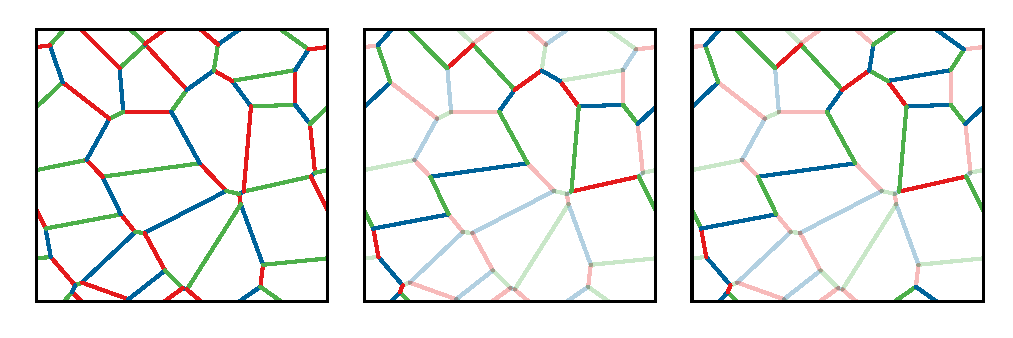
\includegraphics{figure_code/amk_chapter/multiple_colourings/multiple_colourings.pdf}
\caption{Three different valid 3-edge-colourings of amorphous lattices.
Colors that differ from the leftmost panel are
highlighted.}\label{fig:multiple_colourings}
}
\end{figure}

\hypertarget{mapping-between-flux-sectors-and-bond-sectors}{%
\subsection{Mapping between flux sectors and bond
sectors}\label{mapping-between-flux-sectors-and-bond-sectors}}

Constructing the Majorana representation of the model requires the
particular bond configuration \(u_{jk} = \pm 1\). However the large
number of gauge symmetries of the bond sector make it unwieldly to work
with. We therefore need a way to quickly map between bond sectors and
flux sectors.

Going from the bond sector to flux sector is easy since we can compute
it directly by taking the product of \(i u_{jk}\) around each plaquette
\[ \phi_i = \prod_{(j,k) \; \in \; \partial \phi_i} i u_{jk}\]

Going from flux sector to bond sector requires more thought however. The
algorithm I use is this:

\begin{enumerate}
\def\labelenumi{\arabic{enumi}.}
\item
  Fix the gauge by choosing some arbitrary \(u_{jk}\) configuration. In
  practice I use \(u_{jk} = +1\). This chooses an arbitrary one of the 4
  topological sectors.
\item
  Compute the current flux configuration and how it differs from the
  target one. Let's call an plaquette that differs from the target a
  defect.
\item
  Find any adjacent pairs of defects and flip the \(u_jk\) between them.
  This leaves a set of isolated defects.
\item
  Pair the defects up using a greedy algorithm.
\item
  Compute paths along the dual lattice between each pair of plaquettes.
  Flipping the corresponding set of \(u_{jk}\) transports one flux to
  the other and anhilates them.
\end{enumerate}

\begin{figure}
\hypertarget{fig:flux_finding}{%
\centering
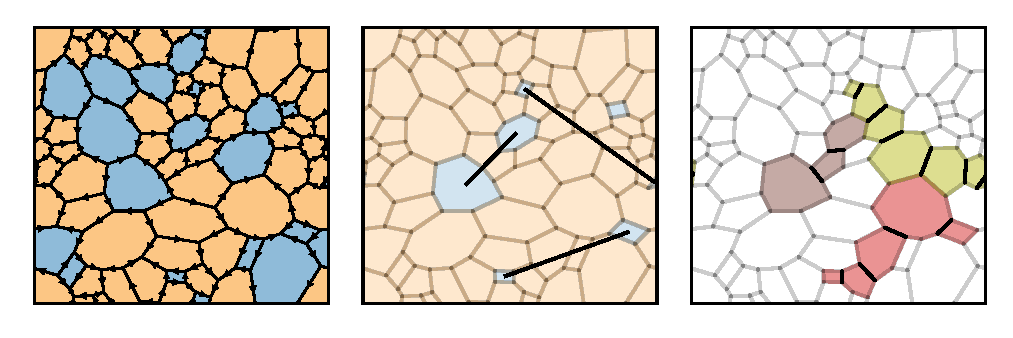
\includegraphics{figure_code/amk_chapter/flux_finding/flux_finding.pdf}
\caption{(Left) The ground state flux sector and bond sector for an
amorphous lattice. Bond arrows indicate the direction in which
\(u_{jk} = +1\). Plaquettes are coloured blue when \(\hat{\phi}_i = -1\)
(\(-i\)) for even (odd) plaquettes and orange when \(\hat{\phi}_i = +1\)
(\(+i\)) for even/odd plaquettes. (Centre) In order to transform this to
the target flux sector (all \(+1\)/\(+i\)) we first flip any \(u_{jk}\)
that are between two fluxes. This leaves a set of isolated fluxes that
need to be anhilated. These are then paired up as indicated by the black
lines. (Right) A* search is used to find paths (coloured plaquettes) on
the dual lattice between each pair of fluxes and the coresponding
\(u_{jk}\) (shown in black) are flipped. One flux has will remain
because the starting and target flux sectors differed by an odd number
of fluxes.}\label{fig:flux_finding}
}
\end{figure}
